\documentclass[12pt, letterpaper]{article}
\usepackage{graphicx}
\graphicspath{ {./images/} }
\title{Visualizing ocean data with Argopy}
\author{Vivek Patel}
\date{June 17, 2021}

\begin{document}

\maketitle

\section{Introduction}
Argopy\footnote{https://github.com/euroargodev/argopy} is an open-source and user-friendly Python package that enables scientists and interested amateurs to analyze and visualize argo ocean datasets.
Ocean are the very important part of our living system and to better understand the system and it is required for scientist to get accurate day to day data. So they created a common platform and collect the ocean data from all around the world. The probes are use to collect the measurement of Pressure, Temperature and Salinity at certain depth and for certain time from the Ocean.

In this project, I tried to apply the computation methods with help of language like Python. The Python is very easy and helpful to conduct such task very efficiently. Also get a chance to apply knowledge of the shell scripting and version control using GIT. By doing some computational tasks, I created intermediate data file from the original data sources and with the help of the intermediate file I created visualization to solve the scientific problems related to dataset.  


\section{Dataset}


To collect data from actual argo model is bit complicated task for the naive users, because it's contain so many models and variables with the ample number of data-lines. But Argopy made this task easy for users it gives you an API with 3 different options to easily collect data. This dataset contains some of the important values such as Latitude, Longitude, Time, Pressure, Temperature and Salinity of the Ocean.




\section{Methodology}


\subsection{Task1}
In the task data was collected for from specific float and converted in to data-frame along with the cleaning and renaming process. Also added some new fields. For this task I tried to process data such as latitude, longitude and temperature. After processing the data it was store in the intermediate .csv file and used to plot a 3D scatter graph. In this scatter graph, I Project latitude on the X-axis, Longitude on the Y-axis and temperature as the depth on Z-axis and color it using the temperature data. The idea behind this plot was to understand the temperature for different latitude and longitude. The visualization for this data is shown in the result section. 

\subsection{Task2}

For the task 2 data was collected for the year 2012 using the API provided by the Argopy. The cleaning and renaming to some of the columns was done before doing major computational task. In the task 2 major data processing was done to achieve mean value of temperature, pressure and salinity for the each month. After completing the all process data was store to intermediate .csv file and by using that file I created the Bar graph for the results. On the Bar graph the X-axis contains the name of months and Y-axis showing the mean value for the temperature, pressure and salinity. The Bar graph provide the clear visualization of the mean value for this three major factors for the all months over the year. Also include the legend to make viewers task more convenient to analyze details from the graph. 


\section{Results}
\subsection{Plot1}

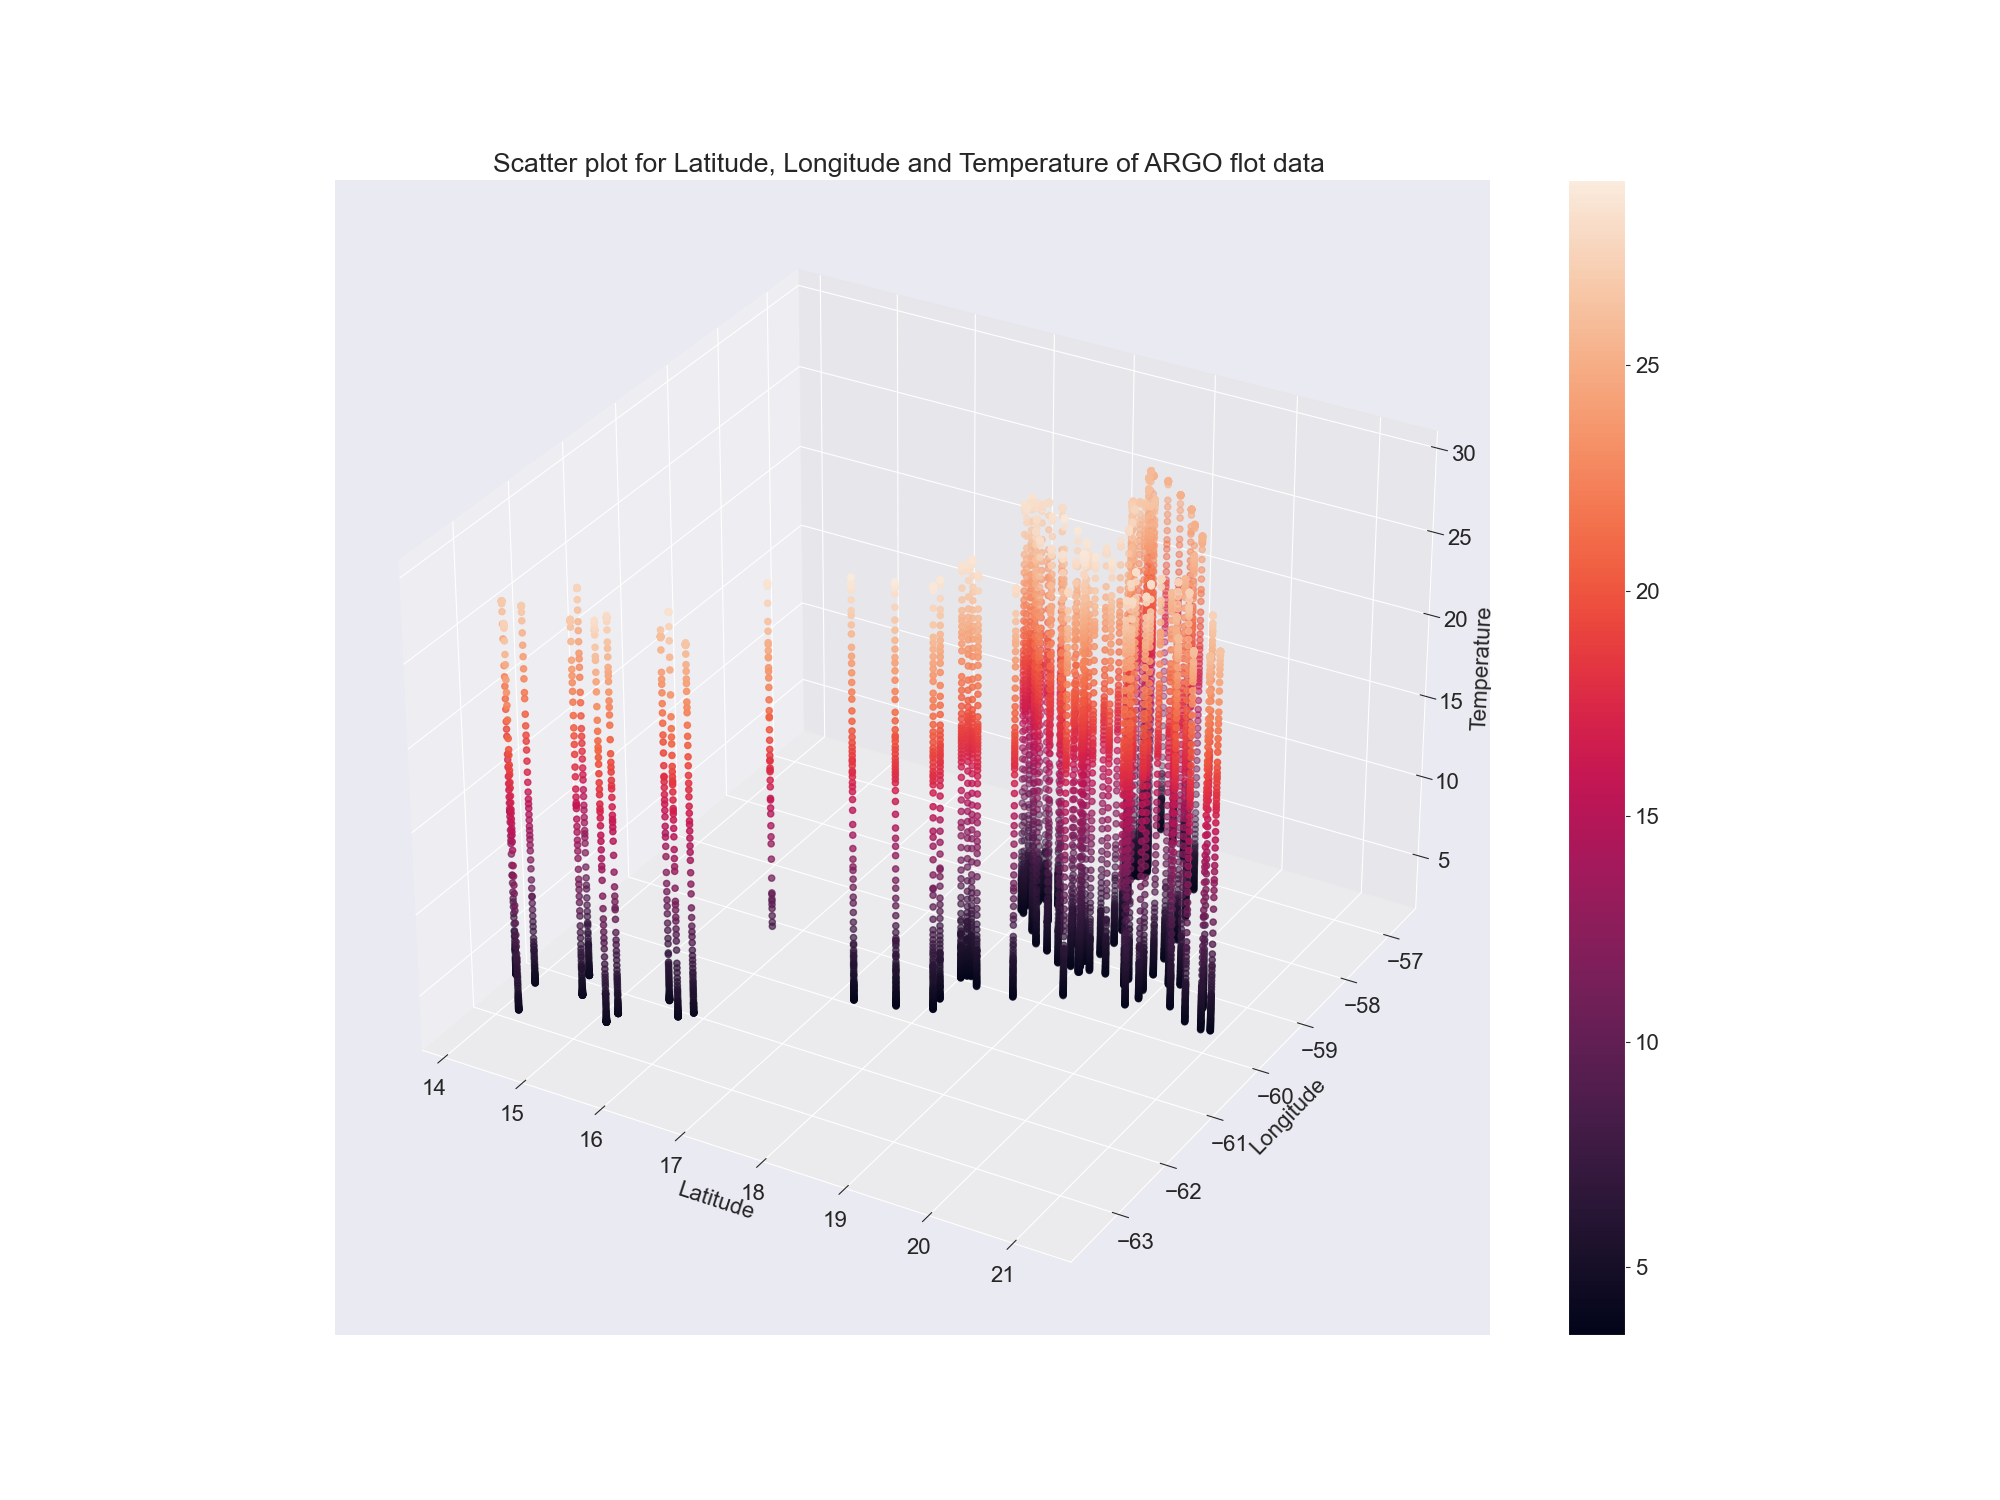
\includegraphics[width=\textwidth]{plot1.png}


\subsection{Plot2}
 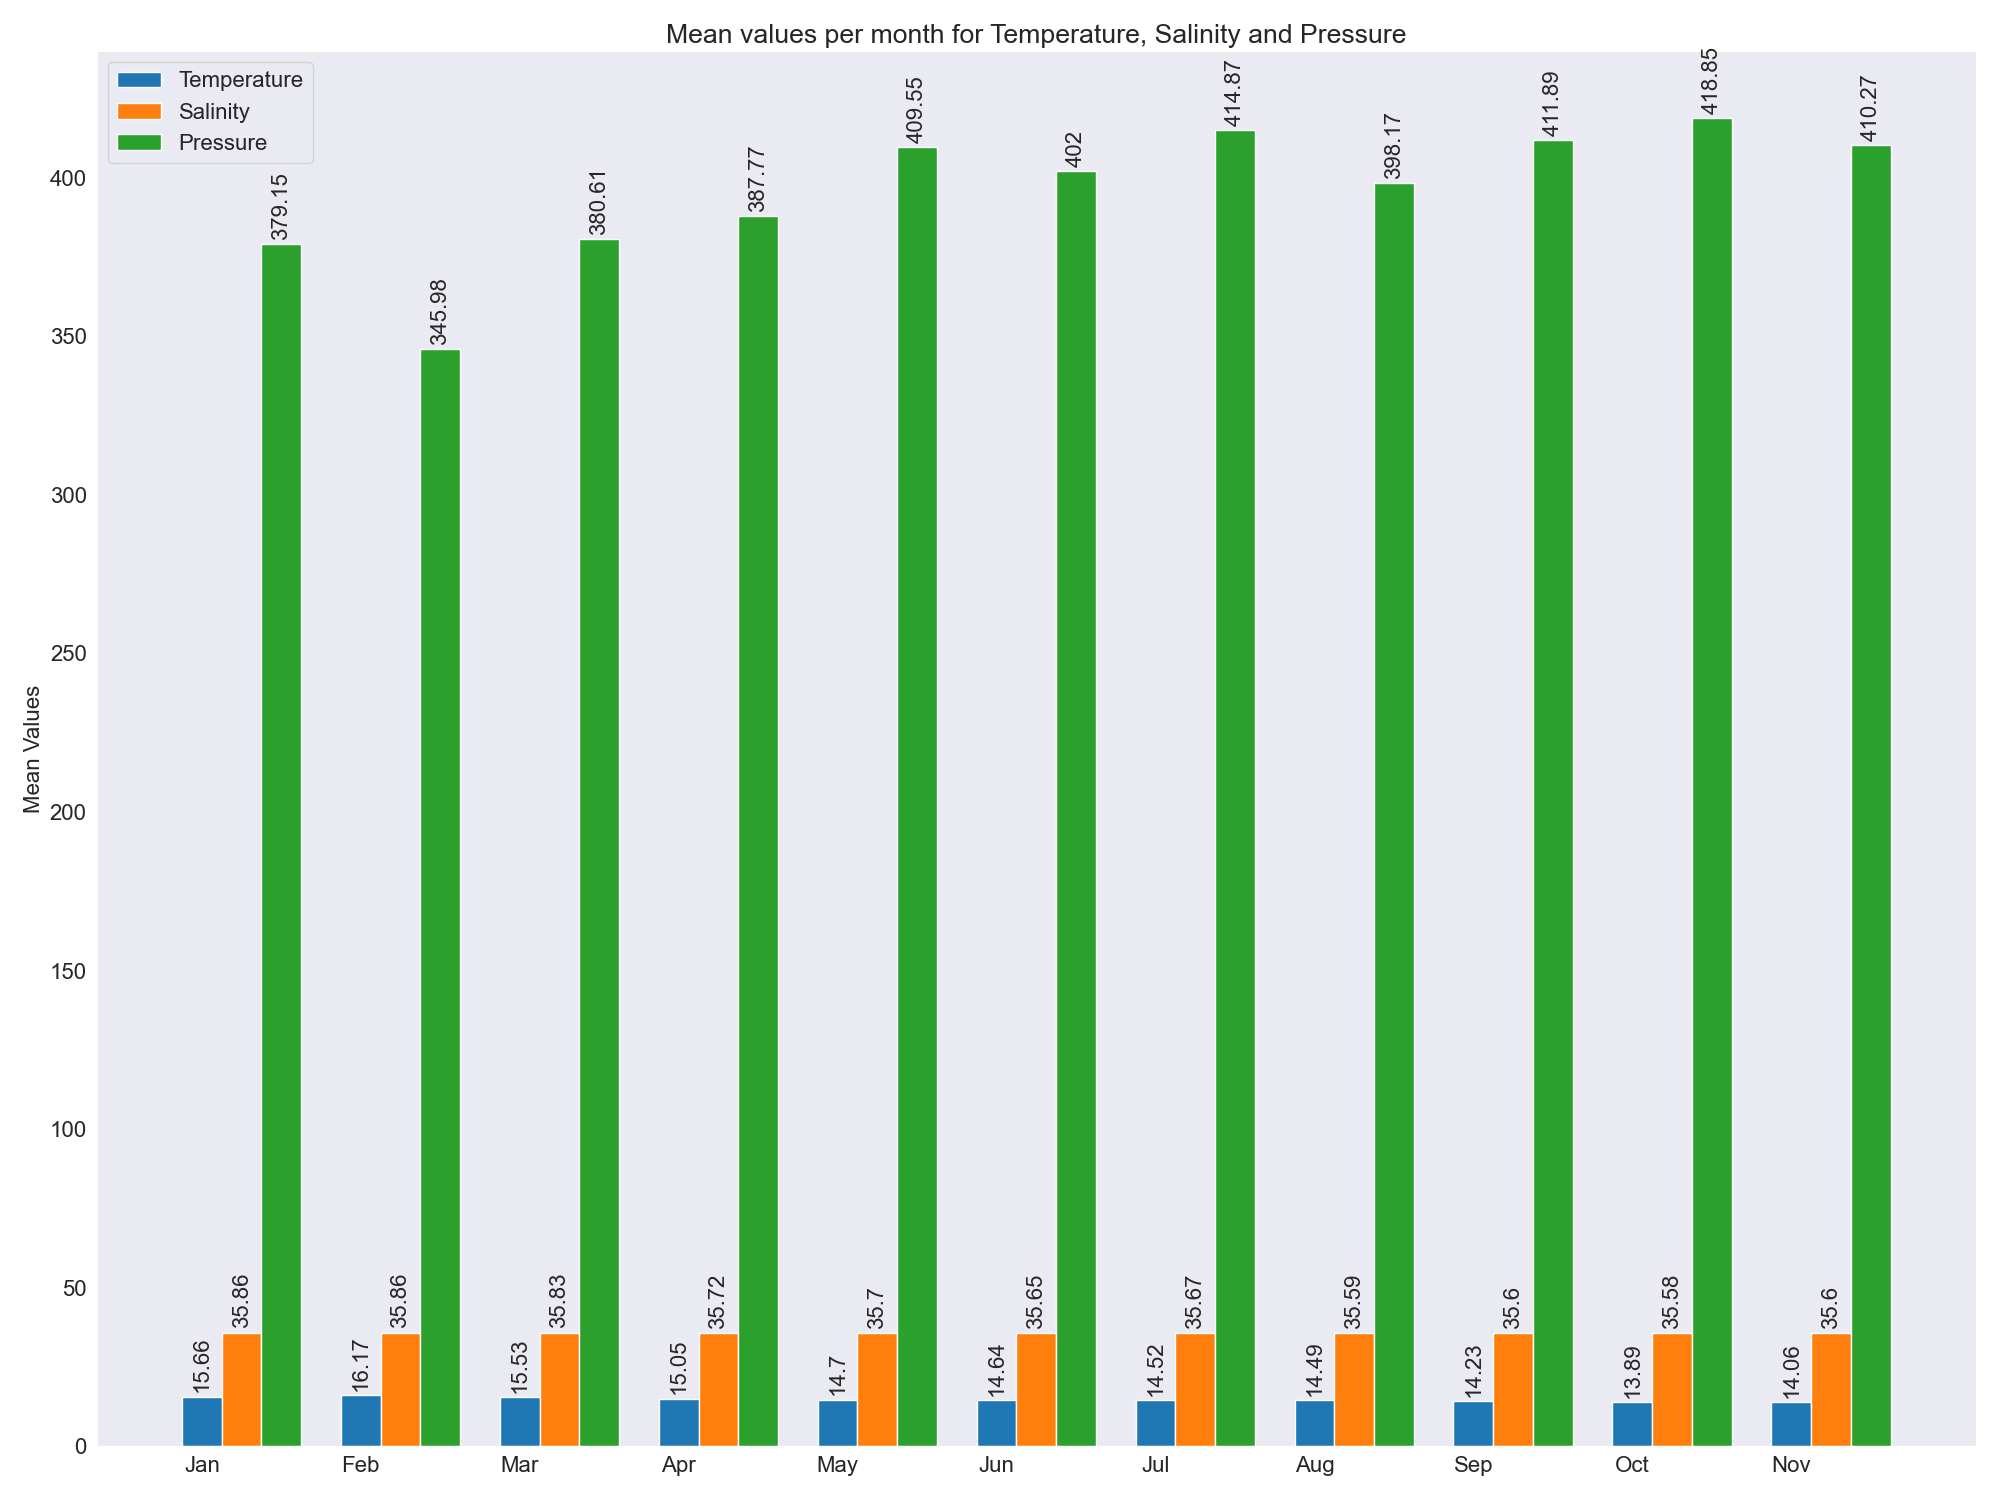
\includegraphics[width=\textwidth]{plot2.png}



\section{Conclusion}

I have tried to explain the usefulness of argopy by plotting two graphs without any prior domain knowledge related to ocean data. Argopy python package is very easy to use and well documented. On top of that I learned the usefulness of python in computational process. Python is very helpful and efficient to handle such task. Also got some experience on version control technology GIT to manage version of project work. Took some basic knowledge about the Latex to create a well formatted document.

I would say by conducting this task I acquired wide range of domain knowledge and understood the usefulness of the python packages to handle various tasks, different other software and other interesting things along with weekly class and assignments work.


\end{document}
